% =========================================================================
\section{Preliminaries}
\label{section:preliminaries}
% =========================================================================

In this section, we present CSP and the concept of minimal hitting set, which
is central to our novel notion of test for failures refinement.

% =========================================================================
\subsection{CSP and Refinement}

%First, we introduce the CSP notation and refinement notions. We then discuss
%a graph-based semantics for finite-state CSP processes.

% =========================================================================
%\subsubsection*{CSP}
%\label{section:CSP}

\subsubsection*{Communicating Sequential Processes (CSP)} is a process algebra
supporting system development by refinement. Using CSP, we model both systems and
their components using processes. They are characterised by their patterns
of interactions, modelled by synchronous, instantaneous, and atomic events.

A prefixing operator $e \then P$ defines a process that is ready to engage in
the event $e$, pending agreement of its environment to synchronise. After $e$
occurs, the process behaves as defined by $P$. The environment can be other
processes, in parallel, or the environment of a system as a whole.

Two forms of choice support branching behaviour. An external choice $P
\extchoice Q$ between processes $P$ and $Q$ offers to the environment the
initial events of $P$ and $Q$. Once synchronisation takes place, the process
that has offered this event is chosen and the other is discarded. In an
internal choice $P \intchoice Q$, the environment does not have an
opportunity to interfere:~the choice is made by the process.
%
\begin{example}\label{example:CSP}
  We consider $P$, $Q$, and $R$ below. $P$ is initially
  ready to engage in the event $a$, and then makes an internal  choice to
  behave like either $Q$ or $R$.
  \begin{eqnarray*}
  P & = & a \then (Q\intchoice R)
  \\
  Q & = & a \then P \extchoice c \then P
  \\
  R & = & b \then P \extchoice c \then R
  \end{eqnarray*}
  $Q$, for instance, offers to the environment the choice to engage in $a$
  again or $c$. In both cases, afterwards, we have a recursion back to $P$.
  In $R$, if $b$ is chosen, we also have a recursion back to $P$. If $c$ is
  chosen, the recursion is to $R$.
  \xbox
\end{example}
%
Iterated forms $\Extchoice i: I @ P(i)$ and $\Intchoice i: I @ P(i)$ of the
external and internal choice operators allow us to define a choice over a
collection of processes $P(i)$. By convention, , if the index set $I$ is
empty, external choices evaluate to the process $\Stop$, which
deadlocks:~does not engage into any event and does not terminate. An iterated
internal choice is not defined for an empty index set.

There are several parallelism operators. A widely used form of parallelism $P
\parallel[cs] Q$ defines a process in which the behaviour is characterised by
those of $P$ and $Q$ in parallel, synchronising on the events in the set
$cs$. Other forms of parallelism available in CSP can be defined using this
operator.

Interactions that are not supposed to be visible to the environment can be
hidden. The operator $P \hide H$ defines a process that behaves as $P$, with
the interactions modelled by events in the set $H$ hidden. Frequently, hiding
is used in conjunction with parallelism:~it is often desirable to make
internal actions of each process in a network of parallel processes, perhaps
used for coordination of the network, invisible, while events happening at
their interfaces remain observable.

A rich collection of process operators allows us to define networks of
parallel processes in a concise and elegant way, and reason about safety,
liveness, and divergences.  A comprehensive account of the notation is given
in~\cite{Roscoe2010}.

A distinctive feature of CSP is its treatment of refinement~(as opposed to
bisimulation), which is convenient for reasoning about program correctness,
due to its treatment of nondeterminism and divergence.  A variety of semantic
models capture different notions of refinement. The simplest model
characterises a process by its possible \emph{traces}; the set $\trc(P)$
denotes the sequences of (non-hidden) events in which $P$ can engage.  We say
that a process \emph{$P$ is trace-refined by another process $Q$}, written $P
\lessdet_T Q$, if $\trc(Q)\subseteq \trc(P)$.

In fact, in every semantic model, subset containment is used to define refinement. The
model we focus on first is the failures model, which captures both
sequences of interactions and deadlock behaviour. A \emph{failure} of a process $P$
is a pair $(s,X)$ containing a trace $s$ of $P$ and a \emph{refusal}:~a set $X$ of
events in which $P$ may refuse to engage, after having performed the events of
$s$. The failures model of a process $P$ records all its failures in a set
$\fails(P)$.

Semantic definitions specify, for each operator, how the traces or failures
of the resulting process can be calculated from the traces or failures of
each operand. For example, for internal choice, $\fails(P\intchoice Q) =
\fails(P)\cup\fails(Q)$; see~\cite[p.~210]{Roscoe:1997:TPC:550448} for a
comprehensive list of these definitions.

Using the notation $P/s$ to denote the process $P$ after having engaged into
trace $s$, the set $\refs(P/s) \defs \{~X | (s,X) \in \fails(P)~\}$ contains
the  refusals of $P$ after $s$. Refusals are
subset-closed~\cite{Hoare:1985:CSP:3921,Roscoe2010}: if $(s,X)$ is a failure
of $P$ and $Y\subseteq X$, then $(s,Y)\in\fails(P)$ and $Y\in\refs(P/s)$
follows.

Failures refinement, $P \lessdet_F Q$, is defined as expected by set
containment $\fails(Q)\subseteq\fails(P)$. Since refusals are subset-closed,
$(s,\varnothing)\in\fails(P)$ for all traces $s\in\trc(Q)$. So, for
divergences-free processes, failures refinement implies trace refinement.
Therefore, using the conformance relation
%
\begin{equation}\label{eq:conf}
  Q\ conf\ P \defs \forall s\in \trc(P) \cap \trc(Q): \refs(Q/s)
  \subseteq \refs(P/s),
\end{equation}
%
failures refinement can be expressed by $\lessdet_T$ and $conf$.
%
\begin{equation}\label{thm:fref-tref-conf}
(P \lessdet_F Q) \iff (P \lessdet_T Q \land Q\ conf\ P)
\end{equation}
%
Throughout this paper, the alphabet of the processes, that is the set of
events that are in scope, is denoted by $\Sigma$ and supposed to be finite.
%Since we are only
%considering ``classical'' CSP processes, the alphabet is always finite.
The FDR tool~\cite{fdr} supports model checking and semantic analyses of
finite-state CSP processes.

For finite CSP processes, since refusals are
subset-closed, $\refs(P/s)$ can be constructed from the set of \emph{maximal
refusals} defined by
%
\begin{equation}
\maxrefs(P/s) = \{ R \in\refs(P/s)~|~\forall R'\in \refs(P/s) - \{ R\}: R \not\subseteq R'\}
\end{equation}
%
Conversely, with the maximal refusals $\maxrefs(P/s)$ at hand, we can
reconstruct the refusals in the set $\refs(P/s)$ as described by
%
\begin{equation}
\refs(P/s) = \{ R'\in\power(\Sigma)~|~\exists R\in \maxrefs(P/s): R'\subseteq R \}.
\end{equation}
%
Deterministic process states $P/s$ have exactly the one maximal refusal
defined by $\Sigma-[P/s]^0$, where $[P/s]^0$ denotes the \emph{initials} of
$P/s$, that is, the events that $P/s$ may engage into. The maximal refusals
in combination with the initials of a process express its degree of
nondeterminism.
%
\begin{example}
\label{ex:nondetdegree} $P = (\Stop \intchoice Q)$ has maximal refusals
$\maxrefs(P) = \{ \Sigma \}$, because $\Stop$ refuses to engage in any event,
and this is carried over to $P$ by the internal choice. However, $P$ is
distinguished from $\Stop$ by its initials, which are defined by $[P]^0 = [
\Stop \intchoice Q]^0 = [Q]^0$. So $P$ may engage nondeterministically in any
initial event of $Q$, but also refuse everything, due to internal selection
of $\Stop$.

Assuming an alphabet $\Sigma = \{a,b,c,d\}$, the process
%
$$Q = (e:\{a,b\} \then \Stop) \intchoice (e:\{c,d\} \then \Stop)$$
%
has maximal refusals $\maxrefs(Q) = \{ \{c,d\}, \{a,b\} \}$ and initials
$[Q]^0=\Sigma$. In contrast to $P$, nondeterminism is reflected by
two maximal refusals. \xbox
\end{example}



% =========================================================================
\subsubsection*{Normalised Transition Graphs for CSP Processes}
\label{sec:ntg}

As shown in~\cite{Roscoe:1994:chapter}, the failures semantics of any
finite-state CSP process $P$ can be represented by a \emph{normalised
transition graph} $G(P)$ defined by a tuple
$$
G(P) = ( N, \ii n, \Sigma, t : N\times\Sigma \pfun N, r : N \fun \mathbb{P}\mathbb{P}(\Sigma)),
$$
with nodes $N$, initial node $\ii n\in N$, and process alphabet $\Sigma$. The
partial \emph{transition function} $t$ maps a node $n$ and an event
$e\in\Sigma$ to its successor node $t(n,e)$. If $(n,e)$ is in the domain of
$t$, then there is a transition, that is, an outgoing edge, from $n$ with
label $e$, leading to node $t(n,e)$. Normalisation of $G(P)$ is reflected by
the fact that $t$ is a function. The graph construction
in~\cite{Roscoe:1994:chapter} implies that all nodes $n$ in $N$ are
reachable by sequences of edges labelled by $e_1\dots e_k$ and connecting
states $\ii n,n_1,\dots,n_{k-1},n$, such that
\[
n_1 = t(\ii n,e_1), \quad n_i = t(n_{i-1},e_i),\ i = 2,\dots,k-1,\quad
n= t(n_{k-1},e_k).
\]
%
By construction, $s\in\Sigma^*$ is a trace of $P$, if, and only if, there is
a path through $G(P)$ starting  at $\ii n$ whose edge labels coincide with
$s$. In analogy to $\trc(P)$, we use the notation $\trc(G(P))$ for the set of
finite, initialised paths through $G(P)$, each path represented by its finite
sequence of edge labels. We note that $\trc(P) = \trc(G(P))$. Since $G(P)$ is
normalised, there is a unique node reached by applying the events from $s$
one by one, starting in $\ii n$. Therefore, $G(P)/s$  is also well defined.
By $[n]^0$ we denote the \emph{initials} of $n$:~the set of events occurring
as labels in any outgoing transitions.
$$
[n]^0 = \{ e\in\Sigma~|~(n,e)\in\dom~t \}
$$
The graph construction from~\cite{Roscoe:1994:chapter} used to define
$G(P)$ for any process $P$ guarantees that $[G(P)/s]^0 = [P/s]^0$ for all
traces $s$ of $P$.

The total function $r$ maps each node $n$ to a non-empty set of  (possibly
empty) subsets of $\Sigma$. The graph construction guarantees that
$r(G(P)/s)$ represents the maximal refusals of $P/s$ for all $s\in\trc(P)$.
As a consequence,
\begin{equation}\label{eq:refsAndR}
(s,X)\in\fails(P) \iff s\in\trc(G(P)) \wedge \exists R\in r(G(P)/s): X\subseteq R,
\end{equation}
so $G(P)$ allows us to re-construct the failures semantics of $P$.
\fixme{alcc: Why not leave the commented out material in the report?}

% Commented out just to shorten the report.
%To see that this approach works only for finite CSP processes, we consider
%the example where $\Sigma$ is infinite. In this case,
%$\maxrefs(\Stop/\langle\rangle)$ is empty, and so we cannot use this set to
%calculate the refusals of $\Stop$, that is, $\refs(\Stop/\langle\rangle)$ as
%defined above. As with refusals, we also use the transition graph-oriented
%notation $\maxrefs(n) \subseteq r(n)$ to denote the maximal refusals
%associated with graph state $n$: if $n$ is the state reached in the
%transition graph by following the edge labels in trace $s$, then $\maxrefs(n)
%= \maxrefs(P/s)$.

% Commented out just to shorten the report.
%Well-formed normalised transition graphs must not refuse an event of the
%initials of a state in {\it every} refusal applicable in this state; more
%formally,
%%
%\begin{equation}
%\label{eq:wellformedg}
%\forall n\in N, e\in\Sigma: (n,e)\in\dom~t \Rightarrow
%\exists R\in r(n): e\not\in R
%\end{equation}
%%
%By construction, normalised transition graphs reflect the \emph{failures
%semantics} of finite-state CSP processes:~the traces $s$ of a process are
%defined by the sequences of transitions associated with paths through its
%graph, starting at $\ii n$. The pairs $(s,R)$ with $s\in\trc(P)$ and $R\in
%r(G(P)/s)$ represent the failures of $P$.

% =========================================================================
\subsubsection*{Acceptances}
\label{sec:accs}

When investigating  tests for failures refinement, the notion of
\emph{acceptances}~\cite{Hennessy:1988:ATP:50497}, which is dual to refusals,
is also useful. An acceptance set of $P/s$ is a subset of its initials
$[P/s]^0$; equivalently, it is a subset of events labelling  outgoing transitions of
$G(P)/s$. If the behaviour of  $P/s$ is deterministic, its only acceptance
equals $[P/s]^0$, because $P/s$ never refuses any of the events contained in
this set. If $P/s$ is nondeterministic, it internally chooses one of its
\emph{minimal acceptance sets} $A$ and never refuses any event in $A$, while
{\it possibly} refusing the events from $[P/s]^0 - A$ and
{\it always} refusing those from $\Sigma - [P/s]^0$.
The acceptances of $P/s$ are denoted by
$\accs(P/s)$, and the minimal acceptances by $\minaccs(P/s)$. They satisfy
the following properties.
%
\begin{eqnarray}
A\in \minaccs(P/s) & \Leftrightarrow & \exists R\in\maxrefs(P/s) \wedge A = \Sigma-R
\label{eq:accref}
\\
\bigcup \{ A~|~A\in \accs(P/s)\} & = & [P/s]^0
\label{eq:accinitials}
\\
 X\in\accs(P/s) &\Leftrightarrow & A\in \minaccs(P/s) \wedge A\subseteq X \subseteq [P/s]^0
 \label{eq:accsubset}
\end{eqnarray}
%
%Note that (\ref{eq:accref}) can be regarded as a definition of minimal
%acceptances by means of maximal refusals. In this case,
%(\ref{eq:accinitials}) and (\ref{eq:accsubset}) are consequences of this
%definition and the fact that refusals are subset-closed. \fixme{alcc: are you
%sure? (4) does not talk about Acc. Is this important?}
%\fixme{jp: I'm sure and I can prove this. However, we don't need this fact, so I suggest to
%removed it.}
%
Exploiting formulas (\ref{eq:accref}), (\ref{eq:accinitials}), and
(\ref{eq:accsubset}), every node of a normalised transition graph can
alternatively be labelled with their minimal acceptances, and this
information is equivalent to that contained in the maximal refusals. Since
process states $P/s$ are equivalently expressed by states $G(P)/s$ of $P$'s
normalised transition graph, we also write $\minaccs(G(P)/s)$ and
note that (\ref{eq:refsAndR}) and (\ref{eq:accref}) imply
\begin{equation}\label{eq:maxrefsminaccs}
\minaccs(G(P)/s) = \{ \Sigma - R | R\in r(G(P)/s) \}.
\end{equation}
\fixme{alcc: proof in the report perhaps?}

% .....................................................................................
 \begin{figure}[t]
   %%\hspace*{-40mm}
   \begin{center}
     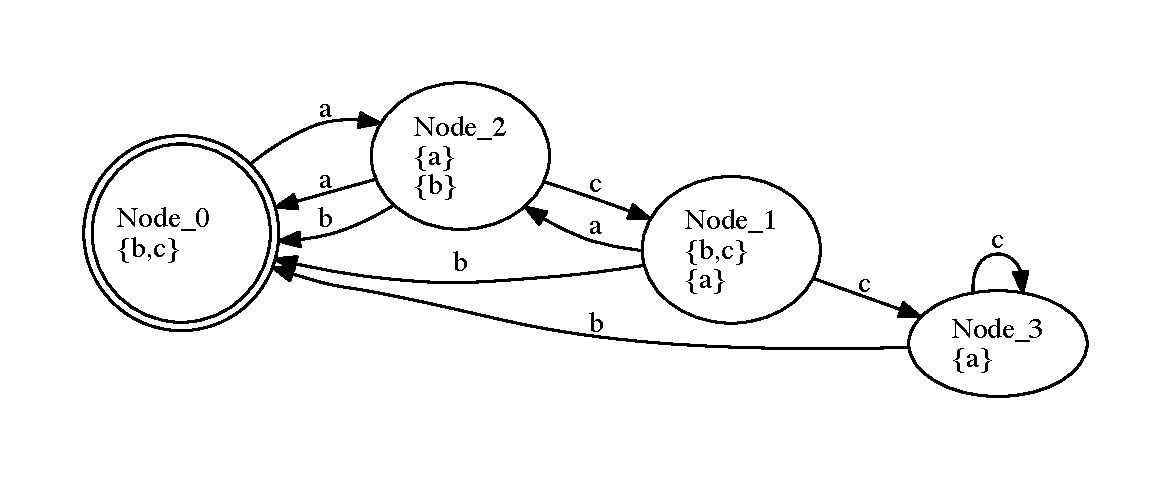
\includegraphics[width=\textwidth]{q0.pdf}
   \end{center}
   %%\vspace*{-10mm}
   \caption{Normalised transition graph of CSP process $P$ from Example~\ref{ex:a}.}
   \label{fig:tga}
 \end{figure}
% .......................................................................................

\begin{example}\label{ex:a}
We consider the process $P$ in Example~\ref{example:CSP}; its transition
graph $G(P)$ is shown in Fig.~\ref{fig:tga}. The process state
$P/\varepsilon$ (where $\varepsilon$ denotes the empty trace) is represented
as Node\_0, with $\{ a\}$ as the only minimal acceptance, since $a$ is never
refused and no other events are accepted. Having engaged in $a$, the
transition from Node\_0 leads to Node\_2 representing the process state $P/a
= Q\intchoice R$. The internal choice induces several minimal acceptances
derived from $Q$ and $R$. Since these processes accept their initial events
in external choice, $Q\intchoice R$ induces minimal acceptance sets $\{a,c\}$
and $\{b,c\}$. We note that the event $c$ can never be refused, since it is
contained in each minimal acceptance set.

Having engaged in $c$, the next process state is represented by Node\_1. Due
to normalisation, there is only a single transition satisfying
$t(\text{Node\_2},c) = \text{Node\_1}$. This transition, however, can have
been caused by either $Q$ or $R$ engaging into $c$, so Node\_1 corresponds to
process state $Q/c \intchoice R/c = P \intchoice R$. This is reflected by the
two minimal acceptance sets labelling Node\_1. Similar considerations explain
the other nodes and transitions in Fig.~\ref{fig:tga}.

Note that the node names including their number suffixes are generated by the
FDR tool. The numbering is generated during the normalisation procedure. So,
the node numbers do not reflect the distance from the initial node Node\_0.
\xbox
\end{example}
%
Summarising, refinement relations between finite-state CSP processes $P, Q$ can be be
expressed by means of their normalised transition graphs
\begin{eqnarray*}
G(P) & = & ( N_P, {\ii n}_P, \Sigma, t_P : N_P\times\Sigma \pfun N_P, r_P : N_P \fun \mathbb{P}\mathbb{P}(\Sigma))
\\
G(Q) & = & ( N_Q, {\ii n}_Q, \Sigma, t_Q : N_Q\times\Sigma \pfun N_Q, r_Q : N_Q \fun \mathbb{P}\mathbb{P}(\Sigma))
\end{eqnarray*}
%
as established by results in the following lemma.
%
\begin{lemma}
  \label{lemma:tgtrcref}
  \begin{eqnarray}
  P \lessdet_T Q & \Leftrightarrow & \trc(G(Q)) \subseteq\trc(G(P))
  \label{eq:trcrefa}
  \\
  \label{eq:failconf}
  P \lessdet_F Q & \Leftrightarrow & P \lessdet_T Q \wedge P\ conf\ Q
  \\
  \label{eq:failrefa}
  P\ conf\ Q & \Leftrightarrow & \nonumber
  \forall s\in\trc(G(Q))\cap \trc(G(P)), R_Q\in r_Q(G(Q)/s):  \nonumber
  \\ & & \tabd
  \exists R_P\in r_P(G(P)/s): R_Q\subseteq R_P
  \\
  \label{eq:failrefb}
   & \Leftrightarrow &
    \forall s\in\trc(G(Q))\cap \trc(G(P)), A_Q\in\minaccs(G(Q)/s):  \nonumber
   \\ & & \tabd
  \exists A_P\in\minaccs(G(P)/s): A_P\subseteq A_Q
 \end{eqnarray}
  \xbox
\end{lemma}
%
The result (\ref{eq:trcrefa}) reflects trace refinement in terms of graph
traces; (\ref{eq:failconf}) expresses failures refinement in terms of traces
refinement and $conf$; (\ref{eq:failrefa}) states how $conf$ can be expressed
by means of the maximal refusal functions of the graphs involved; and
(\ref{eq:failrefb}) states the same in terms of the minimal acceptances that
can be derived from the maximal refusal functions by means of
(\ref{eq:maxrefsminaccs}). \fixme{alcc: I think at least the report should
point to proofs.}

% =========================================================================
\subsubsection*{Reachability Under Sets of Traces}
\label{sec:V} Given a finite-state CSP process $P$ and its normalised
transition graph $G(P)$,
%\[
%G(P) = ( N, \ii n, \Sigma, t : N\times\Sigma \pfun N, r : N \fun \mathbb{P}\mathbb{P}(\Sigma)),
%\]
we suppose that $V\subseteq\Sigma^*$ is a prefix-closed set  of sequences of
events. By $t(\ii n,V)$ we denote the set
\[
t(\ii n,V) = \{ n\in N~|~\exists s\in V: s\in\trc(P)\wedge G(P)/s = n \}
\]
of nodes in $N$ that are reachable in $G(P)$ by applying traces of $V$. The
lemma below specifies a construction method for such sets $V$ reaching {\it
every} node of $N$.

\begin{lemma}
\label{lemma:extendV} Let $P$ be a CSP process with normalised transition
graph $G(P)$. %\fixme{alcc: can a
%normalised graph for a process have states that are unreachable?}
%\fxnote{jp: You are rights: all states in G(P) are reachable by construction of the graph -- I have added this information to the section introducing the graphs.}
Let
$V\subseteq\Sigma^*$ be a finite prefix-closed set of sequences of events.
Suppose that  $G(P)$ reaches $k < |N|$ nodes under $V$, that is, $|t(\ii
n,V)| = k$. Let $V.\Sigma$ denote the set of all sequences from $V$, extended
by any event of $\Sigma$. Then $G(P)$ reaches at least $(k+1)$ nodes under
$V\cup V.\Sigma$.
\end{lemma}
\begin{proof}
Suppose that $n'\in (N - t(\ii n,V))$.  Since all nodes in $N$ are reachable,
there exists a trace $s$ such that $G(P)/s = n'$. Decompose $s = s_1.e.s_2$
with $s_i\in\Sigma^*, e\in\Sigma$, such that $G(P)/s_1 \in t(\ii n,V)$ and
$G(P)/s_1.e \not\in t(\ii n,V)$. Such a decomposition always exists, because
$V$ is prefix-closed and therefore contains the empty trace $\varepsilon$.
Note, however, that it is not necessarily the case that $s_1\in V$.

Since $G(P)$ reaches $G(P)/s_1$ under $V$, there exists a trace $u\in V$ such
that $G(P)/u = G(P)/s_1 = \ol n$. Since $s = s_1.e.s_2$ is a trace of $P$ and
$G(P)/s_1 = \ol n$, then $(\ol n,e)$ is in the domain of $t$. So, $ G(P)/u.e
= G(P)/s_1.e = n$ is a well-defined node of $N$ not contained in $t(\ii
n,V)$. Since $u.e\in V\cup V.\Sigma$, $G(P)$ reaches at least the additional
node $n$ under $V\cup V.\Sigma$. This completes the proof. \xbox
\end{proof}

% =========================================================================
\subsubsection*{Graph Products}
\label{sec:GP}

For proving our main theorems, it is necessary to consider the \emph{product}
of normalised transition graphs. We need this only for the investigation of
corresponding traces in reference processes and processes for SUTs. So, the
labelling of nodes with maximal refusals or minimal acceptances are
disregarded in the product construction. We consider two normalised
transition graphs
\[
G_i = ( N_i, \ii n_i, \Sigma, t_i : N_i\times\Sigma \pfun N_i, r_i : N_i \fun \mathbb{P}\mathbb{P}(\Sigma)),\qquad i = 1,2,
\]
over the same alphabet $\Sigma$. Their product is defined by
%
\begin{eqnarray}
G_1\times G_2 & = & (N_1\times N_2,(\ii n_1,\ii n_2), t:(N_1\times N_2)\times\Sigma\pfun (N_1\times N_2))
\\
\dom~t & = & \{ ((n_1,n_2),e)\in (N_1\times N_2)\times\Sigma~|   \nonumber
\\ & & \tabc
(n_1,e)\in\dom~t_1\wedge
(n_2,e) \in\dom~t_2    \}
\\
t((n_1,n_2),e) & = & (t_1(n_1,e),t_2(n_2,e))\ \text{for $((n_1,n_2),e)\in\dom~t$}
\end{eqnarray}
%
The following lemma is used in the proof of our main theorem.
%
\begin{lemma}\label{lemma:reachproduc}
If $G_1$ has $p$ states and $G_2$ has $q$ states, then every reachable state
$(n_1,n_2)$ of the product graph $G_1\times G_2$ can be reached by a trace
%%%$s\in\trc(G_1)\cap \trc(G_2)$  we don't need this
of maximal length $(pq-1)$.
\end{lemma}
\begin{proof}
The product graph $G_1\times G_2$ has at most $pq$ states. The empty trace $\varepsilon$
reaches its initial state $(\ii n_1,\ii n_2)$. Applying Lemma~\ref{lemma:extendV}
$(pq-1)$ times with $V=\{\varepsilon \}$ implies that $G_1\times G_2$ reaches
all of its reachable states (there are at most $pq$ of them) under
$V' = V \cup V.\Sigma\cup\dots \cup V.\Sigma^{(pq-1)}$. The maximal length of traces in
$V'$ is $(pq-1)$.
\xbox
\end{proof}
\fixme{Abrupt end to the section. It has more than just preliminary material.
It has some new results.}

% =========================================================================
\subsection{Minimal Hitting Sets}
\label{sec:hit}
% =========================================================================

The main idea of the underlying test strategy for failures refinement can be
based on solving a \emph{hitting set problem}. Given a finite collection of
finite sets $C = \{ A_1,\dots,A_n\}$, such that each $A_i$ is a subset of a
universe $\Sigma$, a \emph{hitting set} $H\subseteq\Sigma$ is a set
satisfying the following property.
%
\begin{equation}
  \label{eq:hit}
  \forall A\in C: H\cap A \neq\varnothing.
\end{equation}
%
A \emph{minimal hitting set} is a hitting set that cannot be further reduced
without losing the characteristic property (\ref{eq:hit}). By $\minhits(C)$
we denote the collection of minimal hitting sets for a collection $C$. For
the pathological case where $C$ contains an empty set, $\minhits(C)$ is also
empty.

The problem of determining minimal hitting sets is %%% \cite{Book1975-BOOKRM,5533149}
NP-hard~\cite{5533149}. We see below, however, that it reduces the effort of
testing for failures refinement from a factor of $2^{|\Sigma|}$ to a factor
that equals the number of minimal hitting sets.

The following lemma establishes that the $conf$ relation specified in
(\ref{eq:conf}) can be characterised by means of minimal acceptances and
their minimal hitting sets.
%
\begin{lemma}
\label{lemma:hseta}
Let $P, Q$ be two finite-state CSP processes.
%% satisfying $P\lessdet_T Q$.
For each $s\in\trc(P)$,
let $\minhits(P/s)$ denote the
collection of all minimal hitting sets of $\minaccs(P/s)$.
Then the following statements are equivalent.
\begin{enumerate}
\item $P\ conf\ Q$

\item For all $s\in\trc(P)\cap \trc(Q)$ and $H \in  \minhits(P/s)$, $H$ is
a (not necessariliy minimal) hitting set of $\minaccs(Q/s)$.
\end{enumerate}
\end{lemma}
\begin{proof}
For showing ``$1 \Rightarrow 2$'', assume   $P\ conf\ Q$ and $s\in\trc(P)\cap
\trc(Q)$. Lemma~\ref{lemma:tgtrcref} (\ref{eq:failrefb}), states that
\[
\forall A_Q\in\minaccs(G(Q)/s):
\exists A_P\in\minaccs(G(P)/s): A_P\subseteq A_Q
\]
Therefore, $H \in  \minhits(P/s)$ not only implies $H\cap A_P\neq\varnothing$
for all minimal acceptances $A_P$, but also $H\cap A_Q\neq\varnothing$ for
every minimal acceptance $A_Q$, because $A_P\subseteq A_Q$ for at least one
$A_P$. As a consequence, each $H \in \minhits(P/s)$ is also a hitting set for
$\minaccs(G(Q)/s)$ as required.

To prove ``$2 \Rightarrow 1$'', assume that 2 holds, but that $P\ conf\ Q$
does {\it not} hold. According to Lemma~\ref{lemma:tgtrcref},
(\ref{eq:failrefb}), there exists $s\in\trc(P)\cap \trc(Q)$ such that
\[
\exists A_Q\in\minaccs(G(Q)/s): \forall A_P\in\minaccs(G(P)/s): A_P\not\subseteq A_Q
\qquad (*)
\]
Let $A$ be such an acceptance set $A_Q$ fulfilling (*).
Define
\[
\overline H = \bigcup\{ A_P \setminus A~|~A_P\in\minaccs(G(P)/s) \}.
\]
Since $A_P \setminus A \neq\varnothing$ for all $A_P$ because of (*),
$\overline H$ is a hitting set of $\minaccs(G(P)/s)$ which has an  empty
intersection with $A$.
Minimising $\overline H$ yields   a minimal hitting set $H\in
\minhits(P/s)$ which is {\it not} a hitting set of $\minaccs(G(Q)/s)$, a
contradiction to Assumption~2. This completes the proof of the lemma. \xbox
\end{proof}
%
We note that $\minaccs(P) = \{ \varnothing \}$ if $P = Q\intchoice \Stop$.
Since $\Stop$ accepts nothing, its minimal acceptance is $\varnothing$, and
this carries over to $Q\intchoice \Stop$.  From (\ref{eq:failrefb}) we
conclude that $\varnothing\in\minaccs(P)$ implies $\minaccs(P) = \{
\varnothing \}$. This clarifies that $\minhits(P/s)$ is empty if, and only
if, $\minaccs(P) = \{ \varnothing \}$. The proof of Lemma~\ref{lemma:hseta}
covers the situations where $\minaccs(P/s) = \{ \varnothing \}$ and so
$\minhits(P/s) = \varnothing$.
